\documentclass{examen}

\begin{document}
\modulo{Lenguajes de marcas y sistemas de gesti�n de informaci�n}

Dado el archivo XML que se puede encontrar al final, extraer la informaci�n pedida en los siguientes enunciados usando el lenguaje que se indique

\pregunta{Mostrar la media global de la cantidad de partes suministradas p1, p2 y p4 (Debe salir un solo resultado)}{2}



\pregunta{Averiguar la media de partes suministradas por Jones y Smith (Deben salir dos resultados, la media de Adams y la media de Smith).}{2}
\pregunta{Recuperar los tr�os ``numero de proveedor'', ``numero de parte'', ``n�mero de proyecto'' en los que sus tres ciudades sean distintos}{1}
\pregunta{Recuperar la cantidad de proveedores cuya ciudad es Par�s o su estado es igual o mayor que 20.}{1}


\pregunta{Averiguar la media de cantidades suministrada para proyectos cuya ciudad sea ``Par�s''. El resultado son varias filas}{1}
\pregunta{Indicar cuantos proveedores hay cuyo estado sea 20 y su ciudad sea Londres}{1}
\pregunta{Indicar los c�digos de proyecto que est�n en la misma ciudad que otro proyecto}{2}


\break 
\begin{verbatim}
<datos>
    <proveedores>
        <proveedor numprov="v1">
            <nombreprov>Smith</nombreprov>
            <estado>20</estado>
            <ciudad>Londres</ciudad>
        </proveedor>
        ... omitido ...
    </proveedores>
    <partes>
        <parte numparte="p1">
            <nombreparte>Tuerca</nombreparte>
            <color>Rojo</color>
            <peso>12</peso>
            <ciudad>Londres</ciudad>
        </parte>
        ... omitido ...
    </partes>
    <proyectos>
        <proyecto numproyecto="y1">
            <nombreproyecto>Clasificador</nombreproyecto>
            <ciudad>Paris</ciudad>
        </proyecto>
        ... omitido ...
    </proyectos>
    <suministros>
        <suministra>
            <numprov>v1</numprov>
            <numparte>p1</numparte>
            <numproyecto>y1</numproyecto>
            <cantidad>200</cantidad>
        </suministra>
        <suministra>
            <numprov>v1</numprov>
            <numparte>p1</numparte>
            <numproyecto>y4</numproyecto>
            <cantidad>700</cantidad>
        </suministra>
        ... omitido ...
    </suministros>
</datos>
\end{verbatim}

\break
\begin{figure}[h]
    \caption{Esquema de la base de datos}
    \label{figura1}
    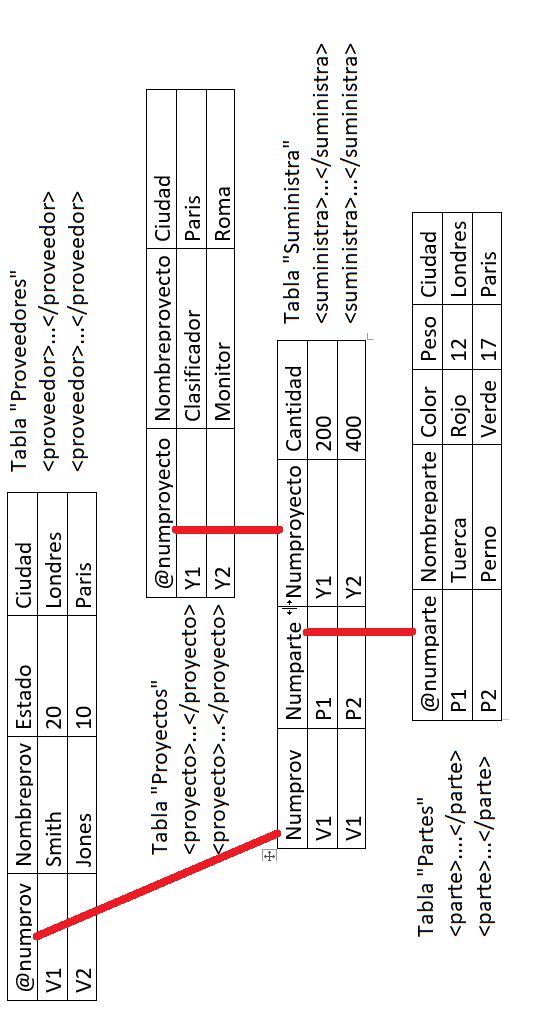
\includegraphics[width=\linewidth]{BaseDatosProveedoresPartesProyectos.png}
\end{figure}

\end{document}
